\documentclass[../statistical_inference.tex]{subfiles}
\begin{document}
\section{Aula 18 - 10 de Fevereiro, 2025}
\subsection{Motivações}
\begin{itemize}
	\item Propriedades lógicas do e-valor.
\end{itemize}
\subsection{Propriedades Lógicas do e-valor}
O primeiro ponto que vamos observar é a lógica composicional por trás das hipóteses avaliadas com o e-valor, começando com uma citação do \textit{Tractatus} de Wittgenstein como inspiração filosófica:
\begin{quote}
	``Numa linguagem razoável, a veracidade ou falsidade de uma sentença completa deve ser logicamente deduzível'',
\end{quote}
que significa essencialmente que valores de verdade de frases complexas devem ser possíveis de se analisar a partir de suas componentes elementares, cujos valores de veracidade são resultados de suas funções-verdade, e todas funções-verdade são resultados de sucessivas aplicações de um número finito de operações-verdade aos constituintes elementares.

A ideia de estudar as propriedades de composicionabilidade nasceu dos pesquisadores intuirem que a álgebra de composicionabilidade do e-valor é muito parecida com a área do estudo de confiabilidade (por exemplo, estudo de tempo de vida de lâmpadas, na qual sabendo a densidade de probabilidade de uma lâmpada num sistema de lâmpadas paralelas, sabemos das outras), ou seja, ela não é nenhuma novidade, mas ela é na área de testagem de hipóteses!
Assim como máquinas na teoria de confiabilidade são construídas a partir das suas contrapartes mais simples, vamos construir os modelos aqui ligando-os em série de vários modelos mais simples, depois compará-los em paralelo, tal qual o diagrama já visto previamente: vamos considerar a sequência de hipóteses alternativas elementares, \(H^{(i, j)},\) com \(i=1,\dotsc ,q\), todas definidas em \(j=1,\dotsc ,k\) modelos constituintes independentes, \(M^{(j)}\), e uma grande hipótese complex H definida pela \textit{composição lógica} na \textit{forma normal homogênea disjuntiva}, ou seja, disjunções de conjunções, das hipóteses elementares no modelo dado pelo produto \(M=M^{(1)\times \dotsc \times M^{(k)}}\), que resulta em
\begin{center}
	\begin{tikzpicture}[
			observed/.style = {rectangle, thick, text centered, draw},
			latent/.style = {ellipse, thick, draw, text centered},
			error/.style ={circle, thick, draw, text centered},
			confounding/.style = {rectangle, thick, text centered, draw, text width = 6em, minimum width = 5.5in},
			outcome/.style = {rectangle, thick, draw, text centered, minimum height = 3.5in, text width = 6em},
		]
		\node[latent](TL) at (-7,0){Origem};
		\node[observed](M_11) at (-3, 3){\(W^{(1),\; s^{*(1,1)}}\)};
		\node[observed](M_12) at (0, 3){\(W^{(2),\; s^{*(1,2)}}\)};
		\node(dt5) at (2,3){\(\cdots\)};
		\node[observed](M_13) at (4, 3){\(W^{(k),\; s^{*(1,k)}}\)};
		\node[observed](M_21) at (-3, 1){\(W^{(1),\; s^{*(2,1)}}\)};
		\node[observed](M_22) at (0, 1){\(W^{(2),\; s^{*(2,2)}}\)};
		\node(dt6) at (2,1){\(\cdots\)};
		\node[observed](M_23) at (4, 1){\(W^{(k),\; s^{*(2,k)}}\)};
		\node(dt1) at (-3,0){\(\vdots\)};
		\node(dt2) at (0,0){\(\vdots\)};
		\node(dt3) at (2,0){\(\ddots\)};
		\node(dt4) at (4,0){\(\vdots\)};
		\node[observed](M_31) at (-3, -1){\(W^{(1),\; s^{*(q,1)}}\)};
		\node[observed](M_32) at (0, -1){\(W^{(2),\; s^{*(q,2)}}\)};
		\node(dt7) at (2,-1){\(\cdots\)};
		\node[observed](M_33) at (4, -1){\(W^{(k),\; s^{*(q,k)}}\)};

		\node[latent](snk) at (7, 0){Sink};

		\draw[Arrow](TL)--node[midway, above] {}(M_11);
		\draw[Arrow](TL)--node[midway, below] {}(M_21);
		\draw[Arrow](TL)--node[midway, left] {}(M_31);

		\draw[Arrow](M_11)--(M_12);
		\draw[Arrow](M_12)--(dt5);
		\draw[Arrow](dt5)--(M_13);

		\draw[Arrow](M_21)--(M_22);
		\draw[Arrow](M_22)--(dt6);
		\draw[Arrow](dt6)--(M_23);

		\draw[Arrow](M_31)--(M_32);
		\draw[Arrow](M_32)--(dt7);
		\draw[Arrow](dt7)--(M_33);

		\draw[Arrow](M_13)--(snk);
		\draw[Arrow](M_23)--(snk);
		\draw[Arrow](M_33)--(snk);

	\end{tikzpicture}
\end{center}
Em termos matemáticos, temos a hipótese H dada por
\[
	H = \bigvee_{i=1}^{q}\bigwedge_{j=1}^{k}H^{(i, j)},
\]
que é o modelo na forma normal disjuntiva (disjunção é uma palavra bonita para ``alternativa''), basicamente indicando que a hipótese complexa é resultante de uma série de disjunção de cláusulas OU's (cláusula 1 OU cláusula 2 OU ...), e cada uma delas é uma conjunção de E's.
Aqui, é até que fácil de analisar os contextos pois podemos escrever com facilidade um modelo geral, afinal sabemos compor os componentes do modelo; por exemplo, o espaço paramétrico \(\Theta \) da H nada mais é que a produtória cartesiana dos espaços paramétricas de cada modelo \(\Theta^{(j)}\); a distribuição \textit{a priori} conjunta pros k-modelos é o produto das distribuições \textit{a priori} de cada modelo, ou seja,
\[
	p_{0} = p_{0}^{(j_1)}\cdot p_{0}^{(j_2)}\dotsc p_{0}^{(j_{k})},
\]
que já nos dá a esperança de calcularmos o e-valor de uma hipótese na forma normal disjuntiva! Outros elementos são obtidos da mesma forma:

Com efeito, o e-valor de uma hipótese na forma normal disjuntiva se calcula como o valor-verdade W no modelo composto, calculada no máximo do produto das funções surpresas em cada produto:
\[
	\mathrm{ev}\biggl(\bigvee_{i=1}^{q}\bigwedge_{j=1}^{k} H^{(i, j)}\biggr) = W\biggl(\max\limits_{1\leq i\leq q} \prod\limits_{j=1}^{k}s^{*(i, j)}\biggr),
\]
onde \(s^{*(i, j)}\) são os máximos elementares e a função-verdade W é dada pela operação-verdade, definida em termos da convolução de Mellin:
\[
	W = \bigotimes_{j=1}^{k}W^{(j)}, \quad W^{(1)}\otimes W^{(2)}(v) = \int_{0}^{\infty}W^{(1)}\biggl(\frac{v}{y}\biggr)W^{(2)}(y) \mathrm{dy},
\]
que consiste na função de densidade de uma variável dada pelo produto aritmética de duas outras variáveis! A convolução de Fourier, por outro lado, dá a densidade de probabilidade da soma aritmética de duas outras variáveis.
Estas operações formam uma álgebra no espaço das funções densidade de probabilidade, tornando possível resolver estas equações algébricas de forma analítica.

A partir disso, vejamos algumas propriedades interessantes: \(\otimes \) é um operador comutativo e associativo; no caso limite, todas as hipóteses \(H^{(i, j)}\), se o e-valor é muito próximo de 0 ou de 1, então a álgebra se reduz à lógica clássica, recuperando o cálculo da lógica clássica da nossa intuição!
Não existe lógica composicional assim para a maior parte de valores-verdade estatísticos, ou seja, para os valores de siginificância, dificultando muito o entendimento dos resultados obtidos por eles; então, o e-valor pode ser caracterizado como uma \textit{medida de possibilidade} obtida por uma transformação da densidade posterior.
Outra caraterística importante é que o cálculo do e-valor consiste em transformar disjunções em produtos e as conjunções tornam-se máximos, que caracterizam um cálculo possibilístico; essa tradução, na verdade, pode ser tratada dentro de um arcabouço unificado onde cada um dos cálculos é caracterizado pela forma que as operações de disjunções e conjunções se traduzem na aritmética normal, ou seja, se tenho eventos disjuntos A e B, a probabilidade de A OU B é traduzida como uma soma, enquanto que, por outro lado, a probabilidade de acontecerem simultaneamente é um produto, traduzindo a conjunção para o produto; na lógica clássica, a disjunção vira o máximo e a conjunção vira o mínimo, e assim segue, segundo a tabela abaixo:
\begin{table}[H]
	\centering
	\caption{Arcabouço de traduções; aqui, \(a = \varphi (A),\; b = \varphi (B),\; c = \varphi (C),\; C = A \wedge B\)}
	\resizebox{\textwidth}{!}{
		\begin{tabular}{c c c c c c c | c}
			\hline
			\(\varphi (\mathcal{U})\) & \(a\oplus b\)   & 0          & 1 & \(a\curlyeqprec b\) & \(c\oslash a\)          & \(a\otimes b\)  & Cálculo         \\
			\hline
			\([0, 1]\)                & a + b           & 0          & 1 & \(a\leq b\)         & \(\frac{c}{a}\)         & \(a \cdot b\)   & Probabilidade   \\
			\([0, 1]\)                & \(\max (a, b)\) & 0          & 1 & \(a\leq b\)         & \(\frac{c}{a}\)         & \(a \cdot b\)   & Possibilidade   \\
			\(\{0, 1\}\)              & \(\max (a, b)\) & 0          & 1 & \(a\leq b\)         & \(\min (c, a)\)         & \(\min (a, b)\) & Lógica Clássica \\
			\([0, 1]\)                & a + b-1         & 1          & 0 & \(b\leq a\)         & \(\frac{(c-a)}{(1-a)}\) & a+b-ab          & Improbabilidade \\
			\(\{0 \dotsc  \infty\}\)  & \(\min (a, b)\) & \(\infty\) & 0 & \(b\leq a\)         & c-a                     & a+b             & Descrença       \\
			\hline
		\end{tabular}}
\end{table}
A \textbf{somatória suporte}, representada pelo operador \(\oplus\), fornece o valor de suporte à disjunção de duas cláusulas logicamente disjuntas, isto é,
\[
	\neg (A \wedge B) \Rightarrow \varphi (A \vee B)=\varphi (A)\oplus\varphi (B),
\]
enquanto que o \textbf{operador de suporte de escala}, \(\oslash\), provém o valor de suporte condicional à afirmação B dada A, a partir dos valores de suporte incondicionais de A e da conjunção \(C = A \wedge B\), ou seja,
\[
	\varphi_{A}(B) = \varphi (A \wedge B)\oslash \varphi (A).
\]

A lógica de possibilidades, por sua vez, caracteriza-se pela tradução das disjunções em operadores de máximo, e conjunções em operador de produto; assim, se todos os valores forem escalares, o valor verdade de a ou b é \(\max\{a, b\}\) e o valor verdade de a e b é \(a \cdot b\), que é exatamente o que aconteceu em
\[
	\mathrm{ev}\biggl(\bigvee_{i=1}^{q}\bigwedge_{j=1}^{k} H^{(i, j)}\biggr) = W\biggl(\max\limits_{1\leq i\leq q} \prod\limits_{j=1}^{k}s^{*(i, j)}\biggr).
\]

Por isso, vamos dar uma aprofundada na lógica modal, onde uma expressão modal é aquela que indica algum grau de avaliação, sendo a mais padrão possível aquela que faz a conta de dois operadores e sua negação; aqui, o operador de possibilidade \(\Diamond\) e o de necessidade \(\square\) são os mais elementares, e \(\neg\) é o operador de negação, que é o contexto do Teste de significância totalmente Bayesiano generalizado (GFBST):
Em muitos casos na vida prática, precisamos pegar uma nota entre 0 e 1, como o e-valor, e traduzir em uma decisão, que idealmente deveria seguir uma linguagem lógica e intuitiva; aqui, isso é dado por:
\begin{itemize}
	\item Rejeitamos H (impossibilidade, \(\neg\Diamond H\) nega a possibilidade de H) se o e-valor está abaixo de uma nota de corte pré-estabelecido, c, ou seja, \(\mathrm{ev}(H)<c\);
	\item Aceitamos H (necessidade, \(\square H\)) se rejeitamos o seu complemento, ou seja, se \(\mathrm{ev}(\overline{H} < c)\); e
	\item Mantemos Agnósticos sobre H, caso contrário (contingência, \(\nabla H = \Diamond H \wedge \neg \square H\)).
\end{itemize}

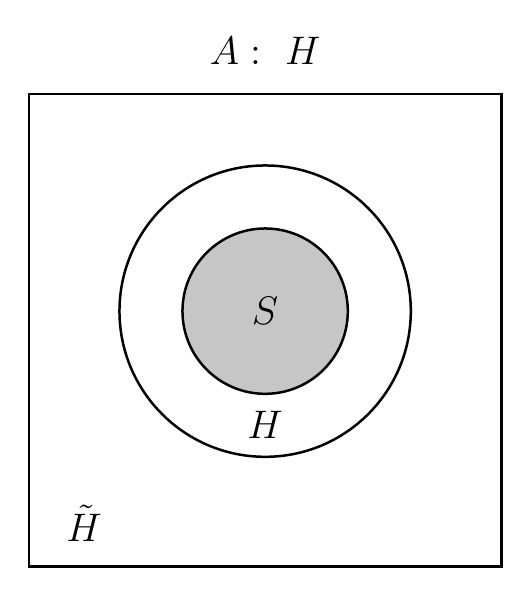
\begin{tikzpicture}[
		x=1cm,y=1cm,
		font=\Large,
		panel/.style={draw, line width=0.9pt},
		set/.style={draw, line width=0.9pt},
		shaded/.style={draw, fill=gray!45, line width=0.9pt},
	]
	\def\W{6}
	% ===================== Panel 1 =====================
	\begin{scope}
		\draw[panel] (0,0) rectangle (\W,\W);
		\node at ({0.5*\W},{\W+0.55}) {$A:\ \square H$};

		% circles
		\draw[set]   ({0.5*\W}, {0.54*\W}) circle[radius=1.85];
		\draw[shaded]({0.5*\W}, {0.54*\W}) circle[radius=1.05];

		% labels
		\node at ({0.5*\W}, {0.54*\W}) {$S$};
		\node at ({0.5*\W}, {0.3*\W}) {$H$};
		\node[anchor=west] at (0.35,0.55) {$\tilde{H}$};
	\end{scope}
\end{tikzpicture}

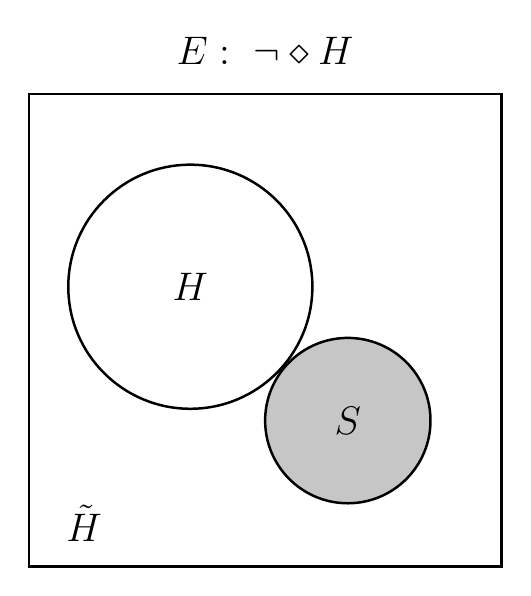
\begin{tikzpicture}[x=1cm,y=1cm,
		font=\Large,
		panel/.style={draw, line width=0.9pt},
		set/.style={draw, line width=0.9pt},
		shaded/.style={draw, fill=gray!45, line width=0.9pt},
	]
	\def\W{6}
	\begin{scope}
		\draw[panel] (0,0) rectangle (\W,\W);
		\node at ({0.5*\W},{\W+0.55}) {$E:\ \neg\diamond H$};

		% circles
		\draw[set]   (2.05,3.55) circle[radius=1.55];
		\draw[shaded](4.05,1.85) circle[radius=1.05];

		% labels
		\node at (2.05,3.55) {$H$};
		\node at (4.05,1.85) {$S$};
		\node[anchor=west] at (0.35,0.55) {$\tilde{H}$};
	\end{scope}
\end{tikzpicture}

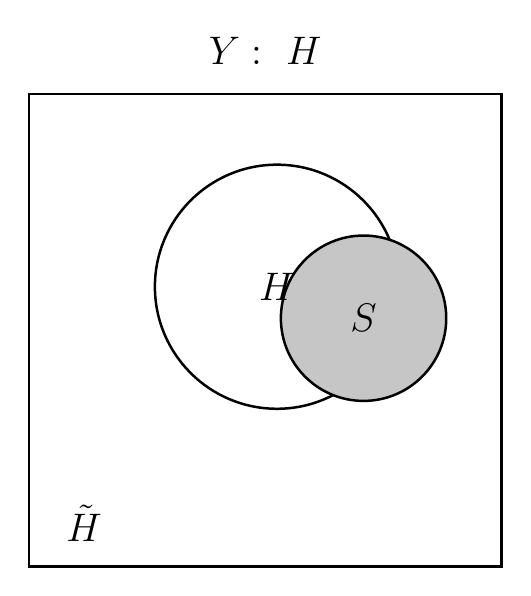
\begin{tikzpicture}[
		x=1cm,y=1cm,
		font=\Large,
		panel/.style={draw, line width=0.9pt},
		set/.style={draw, line width=0.9pt},
		shaded/.style={draw, fill=gray!45, line width=0.9pt},
	]

	\def\W{6}
	% ===================== Panel 3 =====================
	\begin{scope}		\draw[panel] (0,0) rectangle (\W,\W);
		\node at ({0.5*\W},{\W+0.55}) {$Y:\ \triangledown H$};

		% circles
		\draw[set]   (3.15,3.55) circle[radius=1.55];
		\draw[shaded](4.25,3.15) circle[radius=1.05];

		% labels
		\node at (3.15,3.55) {$H$};
		\node at (4.25,3.15) {$S$};
		\node[anchor=west] at (0.35,0.55) {$\tilde{H}$};
	\end{scope}
\end{tikzpicture}

As regras de invertibilidade, monotonicidade e consonância são, aqui,
\begin{itemize}
	\item[I)] \textbf{\underline{Invertibilidade}:} para qualquer hipótese H e seu complemento \(\overline{H} = \Theta -H\), vale
	\item[I.i)] \textbf{Inversão de necessidade}: \(\square H \Longleftrightarrow \neg \Diamond \overline{H}\) (aceitar H é equivalente a negar a possibilidade de não H);
	\item[I.ii)] \textbf{Inversão de possibilidade}: \(\Diamond H \Longleftrightarrow \neq \square\overline{H}\) (a possibilidade de H é equivalente à rejeição da necessidade de não H); e
	\item[I.iii)] \textbf{Inversão de contingência}: \(\nabla H \Longleftrightarrow \nabla \overline{H}\) (a contingência de uma hipótese equivale à contingência de sua negação).

	\item[II)] \textbf{\underline{Monotonicidade}:} para qualquer hipótese H e um superconjunto \(H'\supseteq H\) que contenha H, uma hipótese mais ampla, temos
	\item[II.i)] \textbf{Monotonicidade da necessidade}: \(\square H \Rightarrow \square H'\) (se a hipótese mais forte/restritiva é necessária, então a mais fraca/solta é também); e
	\item[II.ii)]\textbf{Monotonicidade da possibilidade}: \(\Diamond H \Rightarrow \Diamond H'\)  (se a hipótese mais forte é possível, a mais fraca também é).


	\item[III)] \textbf{\underline{Consonância}:} para qualquer conjunto indexado de hipótese \(H^{(i)}, \; i\in I\),
	\item[III.i)] \textbf{Consonância da União:} \(\Diamond (\cup_{i\in I} H^{(i)}) \Rightarrow \exists i\in I:\; \Diamond H^{(i)}\) (se a conjunção de todas as hipóteses é possível, pelo menos uma delas deve ser possível); e
	\item[III.ii)] \textbf{Consonância da Interseção:} \(\forall i\in I, \square H^{(i)} \Rightarrow \square(\cap_{i\in I}H^{(i)})\) (se todas as hipóteses são necessárias, então a interseção delas também é).
\end{itemize}
Podemos representar essas propriedades em termos de diagramas:
\begin{center}
	\begin{tikzpicture}[
			observed/.style = {rectangle, thick, text centered, draw, text width = 6em},
			latent/.style = {ellipse, thick, draw, text centered, text width = 6em},
			error/.style ={circle, thick, draw, text centered},
			confounding/.style = {rectangle, thick, text centered, draw, text width = 6em, minimum width = 5.5in},
			outcome/.style = {rectangle, thick, draw, text centered, minimum height = 3.5in, text width = 6em},
		]

		\node(T) at (0,1){\(\Diamond C\)};
		\node(BL) at (-2,-1){\(\Diamond (A\cup C)\)};
		\node(BR) at (2,-1){\(\Diamond (B\cup C)\)};
		\node(CE) at (0,-2) {};
		\node(BBL) at (-5,-4){\(\Diamond A\)};
		\node(BBR) at (5,-4){\(\Diamond B\)};
		\node(CCE) at (0,-4){\(\Diamond (A\cup B)\)};

		\draw[dashed](T)--node[midway, above] {}(BL);
		\draw[dashed](T)--node[midway, above] {}(BR);
		\draw[dashed](BL)--node[midway, below] {}(CE);
		\draw[dashed](BR)--node[midway, below] {}(CE);
		\draw[blue, -Stealth](CE)--node[midway, right]{\(\Diamond (A\cup B\cup C)\)} (CCE);
		\draw[dashed](BL)--node[midway, above] {}(BBL);
		\draw[dashed](BR)--node[midway, above] {}(BBR);
		\draw[blue, -Stealth](CCE)--(BBL);
		\draw[dashed](CCE)--node[midway, above] {}(BBR);
	\end{tikzpicture}
\end{center}

\begin{center}
	\begin{tikzpicture}[
			observed/.style = {rectangle, thick, text centered, draw, text width = 6em},
			latent/.style = {ellipse, thick, draw, text centered, text width = 6em},
			error/.style ={circle, thick, draw, text centered},
			confounding/.style = {rectangle, thick, text centered, draw, text width = 6em, minimum width = 5.5in},
			outcome/.style = {rectangle, thick, draw, text centered, minimum height = 3.5in, text width = 6em},
		]

		\node(T) at (0,1){\(\neg\Diamond C\)};
		\node(BL) at (-2,-1){\(\neg\Diamond (A\cap C)\)};
		\node(BR) at (2,-1){\(\neg\Diamond (B\cap C)\)};
		\node(CE) at (0,-2) {};
		\node(BBL) at (-5,-4){\(\neg\Diamond A\)};
		\node(BBR) at (5,-4){\(\neg\Diamond B\)};
		\node(CCE) at (0,-4){\(\neg\Diamond (A\cap B)\)};

		\draw[dashed](T)--node[midway, above] {}(BL);
		\draw[dashed](T)--node[midway, above] {}(BR);
		\draw[dashed](BL)--node[midway, below] {}(CE);
		\draw[dashed](BR)--node[midway, below] {}(CE);
		\draw[blue, -Stealth](CE)--node[midway, right]{\(\neg\Diamond (A\cap B\cap C)\)} (CCE);
		\draw[dashed](BL)--node[midway, above] {}(BBL);
		\draw[dashed](BR)--node[midway, above] {}(BBR);
		\draw[blue, -Stealth](CCE)--(BBL);
		\draw[dashed](CCE)--node[midway, above] {}(BBR);
	\end{tikzpicture}
\end{center}

O e-valor satisfaz tudo isso e é uma coisa única para ele, até o momento, finalmente estabelecendo uma ponte entre a filosofia da ciência e a estatística.
\end{document}
